\documentclass[11pt]{article}
\usepackage[margin=1in]{geometry}
\usepackage{amsmath,amssymb,amsthm}
\usepackage{algorithm}
\usepackage{algpseudocode}
\usepackage{tikz}
\usetikzlibrary{arrows.meta}
\usepackage{booktabs}

\title{Column Generation for the Path-Based Maximum Flow Problem}
\author{}
\date{}

\newtheorem{proposition}{Proposition}

\begin{document}
\maketitle

\section{Problem Setup}
Let $G=(V,A)$ be a directed graph with source $s$, sink $t$, and arc capacities $u_a\ge 0$ for $a\in A$. Let $\mathcal{P}$ be the set of all simple $s$--$t$ paths in $G$. For each $p\in\mathcal{P}$ let $f_p\ge 0$ be the flow sent along $p$.

\section{Master Problem (MP)}
\begin{align}
\max\quad & \sum_{p\in\mathcal{P}} f_p \label{mp:obj}\\
\text{s.t.}\quad & \sum_{p\in\mathcal{P}:\, a\in p} f_p \le u_a && \forall a\in A \quad [y_a\ge 0] \label{mp:cap}\\
& f_p \ge 0 && \forall p\in\mathcal{P} \label{mp:dom}
\end{align}

\section{Restricted Master Problem (RMP)}
The RMP is (\ref{mp:obj})--(\ref{mp:dom}) with $\mathcal{P}$ replaced by a subset $\mathcal{P}'\subseteq\mathcal{P}$. Let $y^*$ denote an optimal dual solution of the RMP.

\section{Dual of the Master Problem}
\begin{align}
\min\quad & \sum_{a\in A} u_a\, y_a \\
\text{s.t.}\quad & \sum_{a\in p} y_a \ge 1 && \forall p\in\mathcal{P} \label{dual:path}\\
& y_a \ge 0 && \forall a\in A
\end{align}
Constraint (\ref{dual:path}) is the dual constraint of the column $f_p$; it is violated exactly when the column has positive reduced cost.

\section{Pricing Problem}
The reduced cost of path $p$ is
\begin{equation}
\bar c_p \;=\; 1-\sum_{a\in p} y^*_a .
\end{equation}
A path $p\in\mathcal{P}\setminus\mathcal{P}'$ can improve the RMP if and only if $\bar c_p>0$. Hence the pricing problem is
\begin{equation}
\min_{p\in\mathcal{P}} \; \sum_{a\in p} y^*_a ,
\end{equation}
a shortest $s$--$t$ path problem with arc lengths $y^*_a\ge 0$, solvable by Dijkstra's algorithm.

\begin{proposition}[Optimality]
If the shortest $s$--$t$ path length with respect to $y^*$ is at least $1$, then $y^*$ is feasible for the dual of MP, and the RMP optimal solution is optimal for MP.
\end{proposition}
\begin{proof}
If the shortest path has length $\ge 1$, then $\sum_{a\in p}y^*_a\ge 1$ for every $p\in\mathcal{P}$, so $y^*$ satisfies (\ref{dual:path}) and is dual feasible for MP. Its dual objective equals the RMP optimum, which is the primal value of a feasible MP solution (extend $f$ by zeros). By weak duality both are optimal.
\end{proof}

\section{Algorithm}
\begin{algorithm}[h]
\caption{Column generation for path-based max flow}
\begin{algorithmic}[1]
\State Initialize $\mathcal{P}'$ with at least one $s$--$t$ path (e.g.\ from BFS)
\Loop
  \State Solve the RMP; obtain primal $f$ and duals $y^*$
  \State Run Dijkstra from $s$ to $t$ with arc lengths $y^*$; let $p^*$ be a shortest path
  \If{$\sum_{a\in p^*} y^*_a < 1-\varepsilon$}
    \State $\mathcal{P}'\leftarrow \mathcal{P}'\cup\{p^*\}$
  \Else
    \State \textbf{stop}
  \EndIf
\EndLoop
\State Recover arc flows $x_a=\sum_{p\in\mathcal{P}':\,a\in p} f_p$
\end{algorithmic}
\end{algorithm}

\section{Recovering the Arc Flow and the Cut}
The arc flow
\begin{equation}
x_a=\sum_{p\in\mathcal{P}':\,a\in p} f_p \qquad \forall a\in A
\end{equation}
satisfies $0\le x_a\le u_a$ and flow conservation at all nodes other than $s,t$. By strong duality, the optimal value equals the max-flow value, which equals the minimum cut capacity. The optimal dual $y^*$ is a fractional cut, and a $0/1$ minimum cut can be obtained by thresholding the distance labels $d(v)$ from $s$ (computed w.r.t.\ $y^*$): take $S=\{v: d(v)<\theta\}$ for a suitable $\theta\in[0,1)$.

\section{Worked Example on a 6-Node Network}
Consider the network in Figure~\ref{fig:net} with nodes $V=\{s,a,b,c,d,t\}$ and capacities $u_a$ on the arcs.

\begin{figure}[h]
\centering
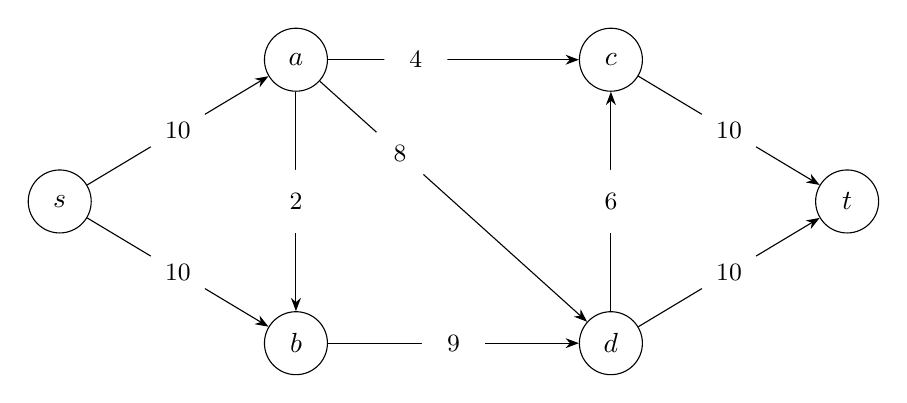
\begin{tikzpicture}[>=Stealth,node distance=2cm,
  every node/.style={circle,draw,minimum size=8mm,inner sep=0pt},
  lab/.style={draw=none,fill=white,inner sep=1pt,font=\small}]
  \node (s) at (0,0) {$s$};
  \node (a) at (3,1.8) {$a$};
  \node (b) at (3,-1.8) {$b$};
  \node (c) at (7,1.8) {$c$};
  \node (d) at (7,-1.8) {$d$};
  \node (t) at (10,0) {$t$};
  \draw[->] (s) -- node[lab] {10} (a);
  \draw[->] (s) -- node[lab] {10} (b);
  \draw[->] (a) -- node[lab] {2} (b);
  \draw[->] (a) -- node[lab,pos=0.35] {4} (c);
  \draw[->] (a) -- node[lab,pos=0.3] {8} (d);
  \draw[->] (b) -- node[lab] {9} (d);
  \draw[->] (d) -- node[lab] {6} (c);
  \draw[->] (c) -- node[lab] {10} (t);
  \draw[->] (d) -- node[lab] {10} (t);
\end{tikzpicture}
\caption{Example network with arc capacities.}\label{fig:net}
\end{figure}

\paragraph{Column generation run.} We start with $\mathcal{P}'=\{P_1\}$, where
\begin{align*}
P_1&=s\to a\to c\to t, & P_2&=s\to a\to d\to t,\\
P_3&=s\to b\to d\to t, & P_4&=s\to a\to d\to c\to t.
\end{align*}
Table~\ref{tab:iter} lists each iteration: the RMP optimum, the duals (only nonzero values shown), and the shortest path found by pricing.

\begin{table}[h]
\centering
\footnotesize
\setlength{\tabcolsep}{4pt}
\begin{tabular}{@{}clllll@{}}
\toprule
It. & $\mathcal{P}'$ & RMP flows $f$ & Obj. & Nonzero duals $y^*$ & Pricing: shortest path (length) \\
\midrule
1 & $P_1$ & $f_1=4$ & 4 & $y_{ac}=1$ & $P_2$ (0), add \\
2 & $P_1,P_2$ & $f_1=2,\ f_2=8$ & 10 & $y_{sa}=1$ & $P_3$ (0), add \\
3 & $P_1,P_2,P_3$ & $f_1=4,\ f_2=1,\ f_3=9$ & 14 & $y_{ac}=y_{dt}=1$ & $P_4$ (0), add \\
4 & $P_1,\dots,P_4$ & $f_1=4,\ f_2=0,\ f_3=9,\ f_4=6$ & 19 & $y_{sa}=y_{bd}=1$ & $P_1$ (1), \textbf{stop} \\
\bottomrule
\end{tabular}
\caption{Column generation iterations. Dual solutions need not be unique; the values shown are those returned by one LP solver run.}\label{tab:iter}
\end{table}

\paragraph{Result.} At iteration 4 the shortest path has length $1\ge 1$, so no column has positive reduced cost and the RMP is optimal for MP. The maximum flow value is $19$, with arc flows
\[
x_{sa}=10,\ x_{sb}=9,\ x_{ac}=4,\ x_{ad}=6,\ x_{ab}=0,\ x_{bd}=9,\ x_{dc}=6,\ x_{ct}=10,\ x_{dt}=9 .
\]
The final dual $y^*_{sa}=y^*_{bd}=1$ is the indicator of the cut $\delta^+(\{s,b\})=\{(s,a),(b,d)\}$ (arc $(a,b)$ goes into $\{s,b\}$ and does not count), whose capacity is $10+9=19=\sum_a u_a y^*_a$, certifying optimality.

\section{Extension: Constrained Paths}
If admissible paths must satisfy side constraints, the master problem is unchanged and only the path set in the pricing problem changes to $\mathcal{P}_{\text{feas}}\subseteq\mathcal{P}$. For example:
\begin{itemize}
  \item \textbf{Hop limit $H$:} $\min_{p\in\mathcal{P},\,|p|\le H}\sum_{a\in p}y^*_a$ (hop-constrained shortest path, e.g.\ Bellman--Ford with $H$ iterations).
  \item \textbf{Resource limit:} $\sum_{a\in p} r_a\le R$ gives a resource-constrained shortest path problem, solved by labeling or dynamic programming.
\end{itemize}
In the constrained case the termination test is unchanged: stop when the constrained shortest path has length $\ge 1$.

\end{document}
